\section{Combined Model} \label{sec:CombinedModel}
In the following section an overview of the chapter is given. The found models, i.e. the attitude and translational model of the system, is presented with the constituted non-linear equations following the same equations linearized. Hereafter, to give the reader a better overview, two block diagrams illustrating the linearized equations are displayed. In the last part of the section the two models are simulated, this aims to analyze the angular and translational behavior. The simulation is also used to see if the linear approximation of the equations gives a valid result compared to the non-linear equations.

\subsection{Attitude Model Equations}
\begin{itemize}
	\item Non-linear equations
	\begin{align}
		J_x\cdot\ddot{\phi}&=k_{th} \cdot(\omega^2_4-\omega^2_2) \cdot L\label{eq:AngleEqVelocitiescombined1}\\
		J_y \cdot\ddot{\theta}&=k_{th} \cdot(\omega^2_1-\omega^2_3) \cdot L\label{eq:AngleEqVelocitiescombined2}\\
		J_z\cdot\ddot{\psi}&=k_d \cdot(\omega^2_1-\omega^2_2+\omega^2_3-\omega^2_4)
		\label{eq:AngleEqVelocitiescombined3}
	\end{align}
	\item Linearized equations
	\begin{flalign}
		J_x\cdot\Delta\ddot{\phi}   &= 2 \cdot k_{th} \cdot L \cdot({\overline{\omega}_4}\cdot \Delta \omega_2-{\overline{\omega}_2}\cdot \Delta \omega_4) \\
		J_y\cdot\Delta\ddot{\theta} &= 2 \cdot k_{th} \cdot L \cdot({\overline{\omega}_1}\cdot \Delta \omega_1-{\overline{\omega}_3}\cdot \Delta \omega_3) \\
		J_z\cdot\Delta\ddot{\psi}   &= 2 \cdot k_d \cdot ({\overline{\omega}_1}\cdot \Delta \omega_1-{\overline{\omega}_2}\cdot \Delta \omega_2+{\overline{\omega}_3}\cdot \Delta \omega_3-{\overline{\omega}_4}\cdot \Delta \omega_4)
	\end{flalign} \label{eqAngleLincombined}
\end{itemize}

\subsection{Translational Model Equations}
\begin{itemize}
	\item Non-linear equations
	\begin{flalign}
		\eq{m\cdot\ddot{x}_I}{-k_{th}\cdot({\omega_1}^2+{\omega_2}^2+{\omega_3}^2+{\omega_4}^2)\cdot\sin(\theta)} \label{eq:AccelerationEqInertialVelocitiescombined1}\\
		\eq{m\cdot\ddot{y}_I}{-k_{th}\cdot({\omega_1}^2+{\omega_2}^2+{\omega_3}^2+{\omega_4}^2)\cdot(-\sin(\phi))\cdot\cos(\theta)} \label{eq:AccelerationEqInertialVelocitiescombined2}\\
		\eq{m\cdot\ddot{z}_I}{F_g-k_{th}\cdot({\omega_1}^2+{\omega_2}^2+{\omega_3}^2+{\omega_4}^2)\cdot\cos(\phi)\cdot\cos(\theta)}
		\label{eq:AccelerationEqInertialVelocitiescombined3}
	\end{flalign}
	\item Linearized equations 
	\begin{flalign}
		m\cdot\Delta\ddot{x}_I &= -k_{th}\cdot({\overline{\omega}_1}^2+{\overline{\omega}_2}^2+{\overline{\omega}_3}^2+{\overline{\omega}_4}^2)\cdot\cos(\overline{\theta})\Delta\theta &\\
		m\cdot\Delta\ddot{y}_I &=  k_{th}\cdot({\overline{\omega}_1}^2+{\overline{\omega}_2}^2+{\overline{\omega}_3}^2+{\overline{\omega}_4}^2)\cdot\cos(\overline{\phi})\cdot\cos(\overline{\theta})\cdot\Delta\phi &\\
		m\cdot\Delta\ddot{z}_I &= -2\textbf{ }k_{th}\cdot({\overline{\omega}_1}\cdot\Delta\omega_1+{\overline{\omega}_2}\cdot\Delta\omega_2+{\overline{\omega}_3}\cdot\Delta\omega_3+{\overline{\omega}_4}\cdot\Delta\omega_4)\cdot\cos(\overline{\phi})\cdot\cos(\overline{\theta})
	\end{flalign} \label{eq:FinalLinearEquationscombined}
\end{itemize}

\subsection{Linearized Block Diagrams}
The block diagrams of the linear approximated attitude and translational equations are illustrated in \autoref{fig:LinearModelBlockDiagram} and \ref{fig:TranslationalLinearModelBlockDiagram}.
\begin{figure}[H]
	\centering
	\includegraphics[scale=0.45]{figures/LinearModelBlockDiag.pdf}
	\caption{A block diagram of the attitude model linear approximated equations. The input is the angular velocities of the four motors and the output is the three angles roll, pitch and yaw.}
	\label{fig:LinearModelBlockDiagram}
\end{figure}
\begin{figure}[H]
	\centering
	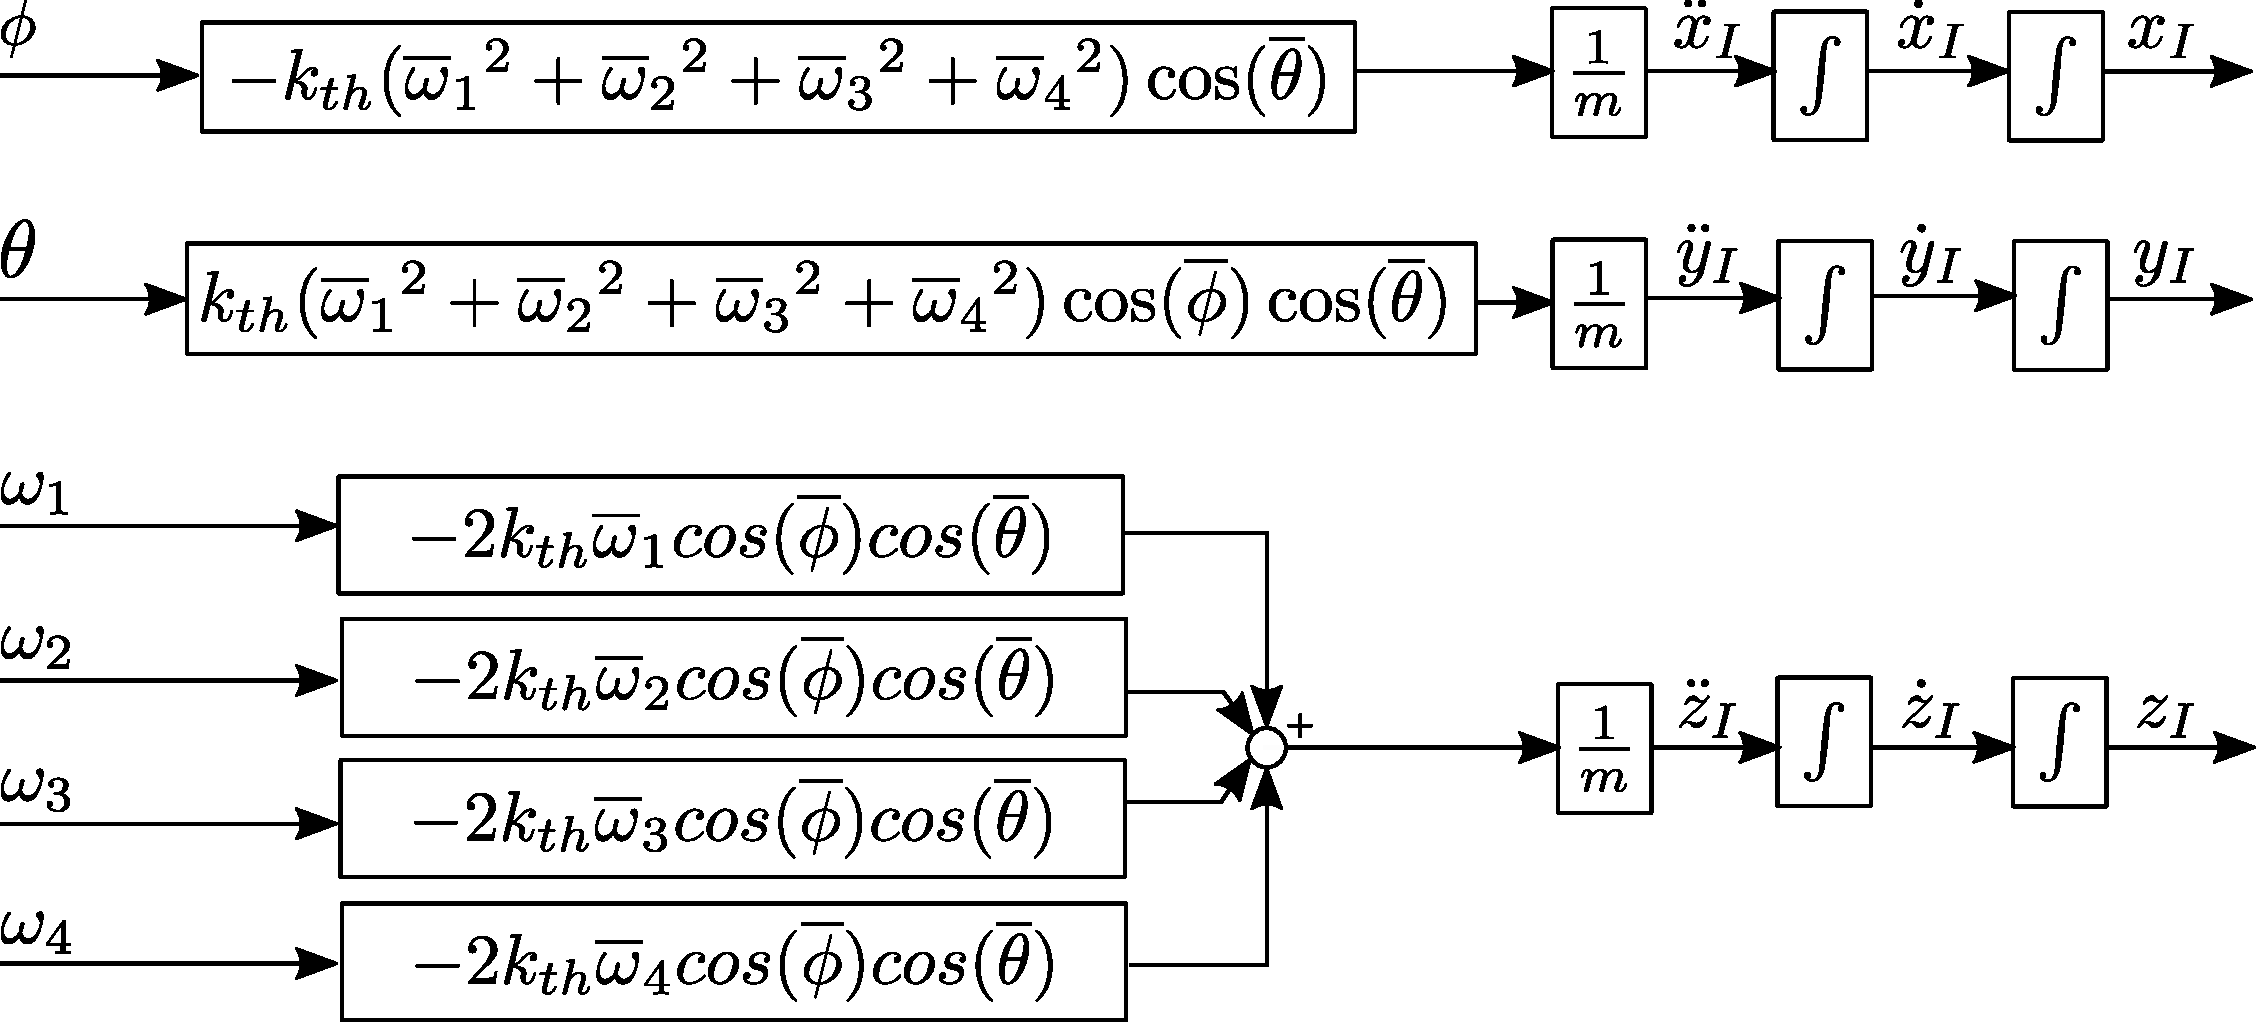
\includegraphics[scale=0.45]{figures/TranslationalLinearModelBlockDiagram.pdf}
	\caption{A block diagram of the translational model linear approximated equations. The input is the angular velocities of the four motors and the output is the three positions in x, y and z.}
	\label{fig:TranslationalLinearModelBlockDiagram}
\end{figure}

\subsection{Simulation}
The simulation of the model is done in Simulink. The parameters used for the simulations are shown in \autoref{ParametersQuadcopter}.
\begin{table}[H]
	\centering
	\begin{tabular}{|l|l|l|p{3cm}|}
		\hline %-----------------------------------------------------------------------------------
		\textbf{Parameter Name}&\textbf{Symbol} &\textbf{Value} &\textbf{Units}\\
		\hline %-----------------------------------------------------------------------------------
		Mass of the quadcopter  & $m$ & 0.996       &$kg$\\
		\hline
		%-----------------------------------------------------------------------------------
		Moment of inertia around x axis       & $J_x$  & 0.01073       & $kg \cdot m^2$\\
		\hline %-----------------------------------------------------------------------------------
		Moment of inertia around y axis       & $J_y$  & 0.01073       & $kg \cdot m^2$\\
		\hline %-----------------------------------------------------------------------------------
		Moment of inertia around z axis       & $J_z$  & 0.02135       & $kg \cdot m^2$\\
		\hline %-----------------------------------------------------------------------------------
		Length of quadcopter arm       & $L$  &   0.225       & $m$\\
		\hline %-----------------------------------------------------------------------------------
		Thrust force constant       & $k_{th}$  & -       & $N\cdot s^2 rad^{-2}$\\
		\hline %-----------------------------------------------------------------------------------\\
		Drag torque constant      & $k_{d}$  & -       & $Nm\cdot m^2 rad^{-2}$\\
		\hline %-----------------------------------------------------------------------------------\\
	\end{tabular}
	\caption{Parameters used in the simulation of the model.}
	\label{ParametersQuadcopter}
\end{table}\vspace{-18pt}

\subsubsection{Attitude Model Simulations}
In \autoref{fig:rollCompModel}, \ref{fig:pitchCompModel} and \ref{fig:yawCompModel}, the angular behavior of the model is analyzed. The input to the system are the four motor velocities. They are defined so the response of the model is predictable and the its performance can be evaluated.

The behavior around x axis is shown in \autoref{fig:rollCompModel}. Only the speeds of motors 2 and 4 are changed as they are supposed to be the ones that affect the roll angle. It can be seen that a positive difference in the rotation speed of these motors generates a positive acceleration in the roll direction, which is consistent with \autoref{eq:AngleEqVelocitiescombined1}.

It can also be observed that the linear approximation of the equations yields an accurate result as the two responses show no perceptible difference. 
%
\begin{figure}[H]
	\centering
	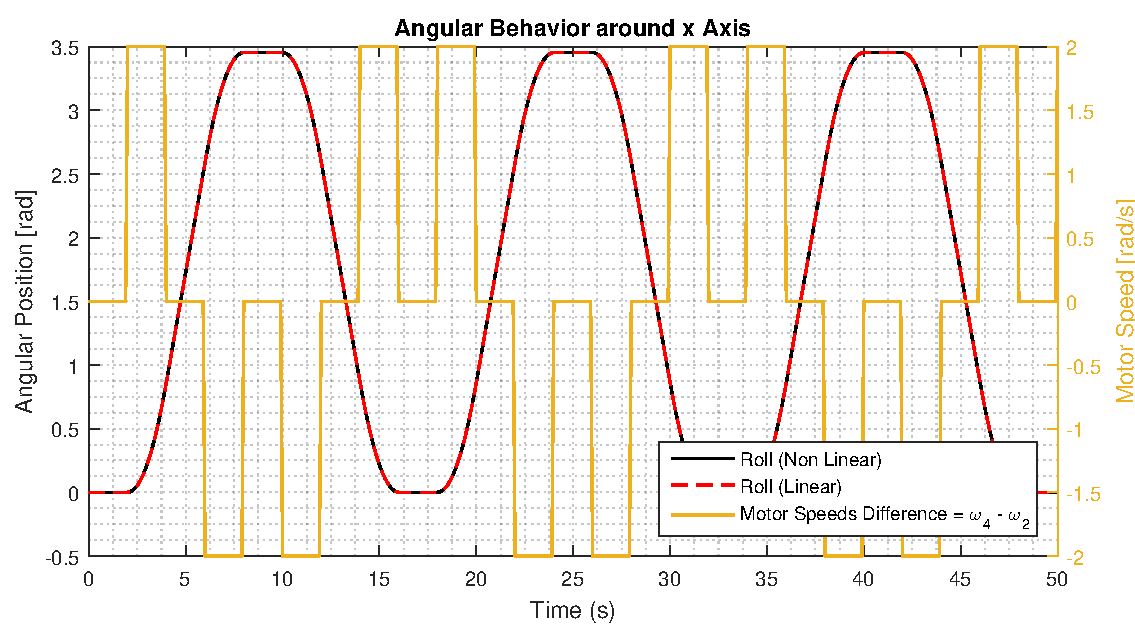
\includegraphics[scale=0.65]{figures/rollCompModel}
	\caption{Behavior of the non linear and linear models in roll angle.}
	\label{fig:rollCompModel}
\end{figure}
%
The behavior around the y axis is very similar to that of the roll angle. It is shown in \autoref{fig:pitchCompModel}. In this case, the motor velocities modified are those from motors 1 and 3. 
%
\autoref{eq:AngleEqVelocitiescombined2} states that a positive rotational speed difference creates a positive pitch acceleration. This is confirmed by the simulations in both models. Again, the linear approximation can be considered adequate.
\begin{figure}[H]
	\centering
	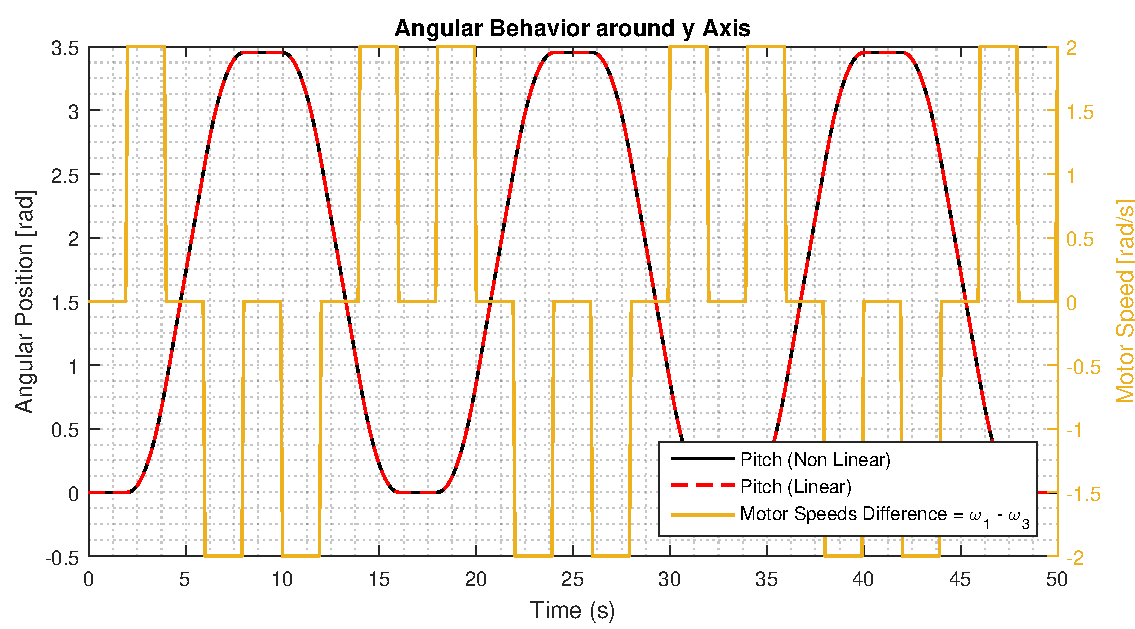
\includegraphics[scale=0.65]{figures/pitchCompModel}
	\caption{Behavior of the non linear and linear models in pitch angle.}
	\label{fig:pitchCompModel}
\end{figure}
%
The last attitude response simulated is around the z axis and is displayed in \autoref{fig:YawCompModel}. In this case all motor velocities affect the yaw angle. In the simulation, velocities of motors 1 and 3 are increased while those of motors 2 and 4 are decreased and vice versa. This creates yaw accelerations according to \autoref{eq:AngleEqVelocitiescombined3}. The response of the model is also correct and the linear approximation can be said to be accurate. 
%
\begin{figure}[H]
	\centering
	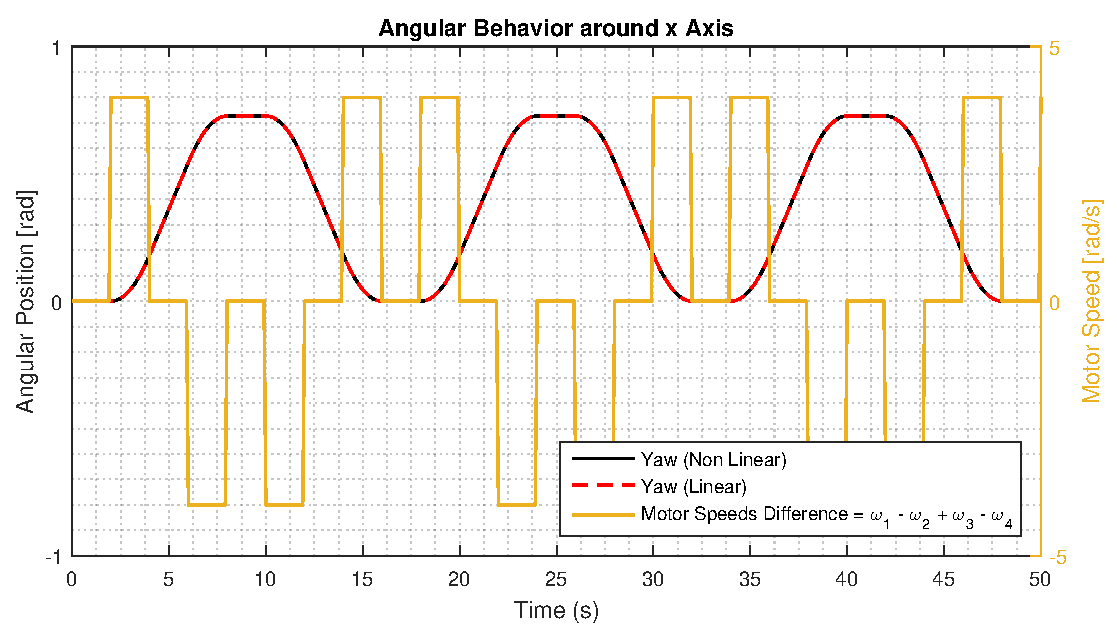
\includegraphics[scale=0.65]{figures/yawCompModel}
	\caption{Behavior of the non linear and linear models in yaw angle.}
	\label{fig:yawCompModel}
\end{figure}

\subsubsection{Translational Model Simulations}
The simulations carried out in the translational models are shown in  \autoref{fig:xCompModel}, \ref{fig:yCompModel} and \ref{fig:zCompModel}. The inputs for these model are roll and pitch angles and the addition of the four motor velocities. 

\autoref{fig:xCompModel} shows how the inertial position in the x axis evolves with constant velocities of the motors and a change in the pitch angle. As expected, a negative translational acceleration is generated for a positive angle change and that drives the position to negative values. This response follows \autoref{eq:AccelerationEqInertialVelocitiescombined1}. The linear approximation is considered suitable when looking at the linear model response.
\begin{figure}[H]
	\centering
	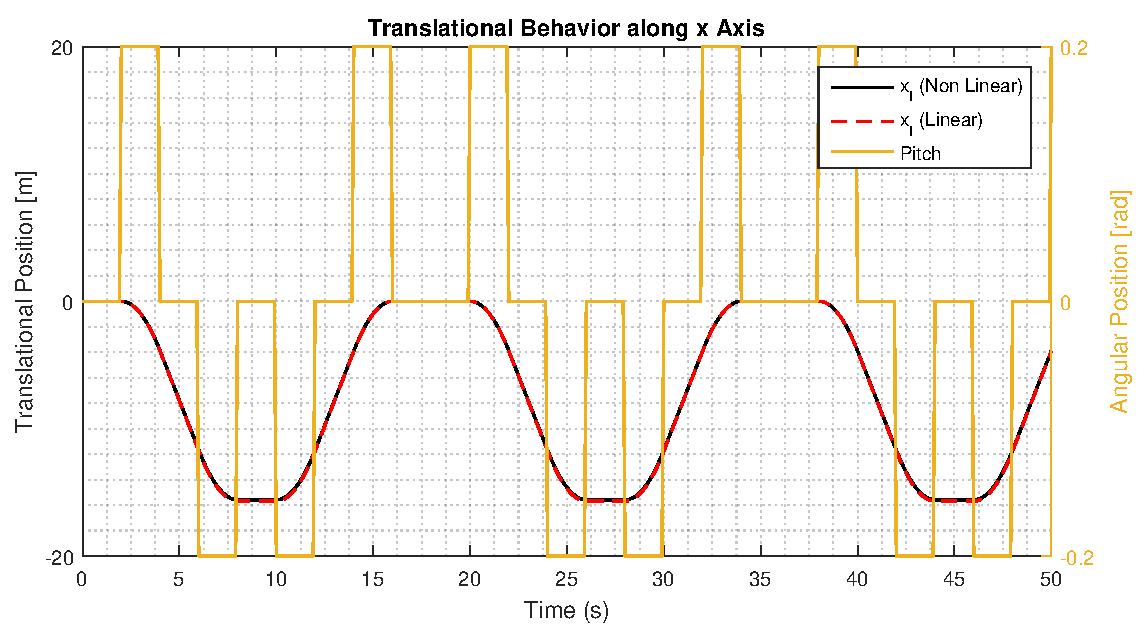
\includegraphics[scale=0.65]{figures/xCompModel}
	\caption{Behavior of the non linear and linear models along the x axis.}
	\label{fig:xCompModel}
\end{figure}
The response along the y inertial direction is depicted in \autoref{fig:yCompModel}. It is similar to that of the x direction but in this case a change in roll is needed to change the acceleration. Now, a positive roll angle generates a positive acceleration, as opposed to the x axis case. All goes in accordance with \autoref{eq:AccelerationEqInertialVelocitiescombined2}. As previously, the linear approximation performs well in the simulation.
\begin{figure}[H]
	\centering
	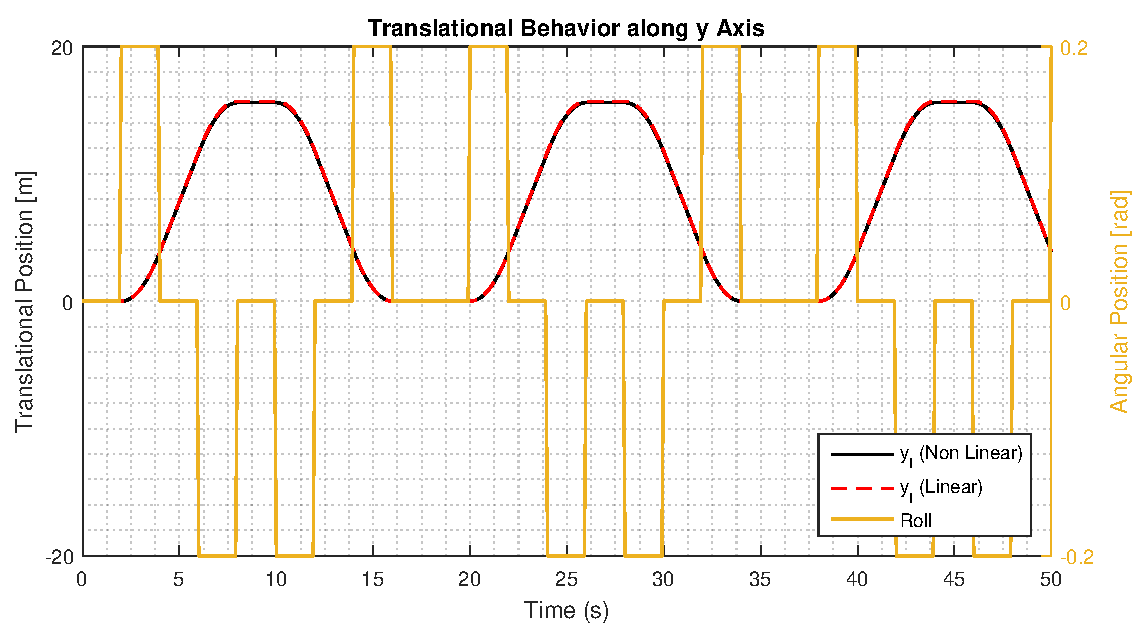
\includegraphics[scale=0.65]{figures/yCompModel}
	\caption{Behavior of the non linear and linear models along the y axis.}
	\label{fig:yCompModel}
\end{figure}
Finally, \autoref{fig:zCompModel} presents the behavior along the z axis. The pitch and roll angle are kept to zero and the summation of motor velocities are changed. For a higher sum, a more negative acceleration in the z axis is generated as it can be seen in \autoref{eq:AccelerationEqInertialVelocitiescombined3} and in the simulation through the z position. In this case, the linear approximation of the squared velocity term in the equations creates a difference in the output z position between the two models that is noticeable in the graph. This difference can be considered not to affect the system as the controller designed will handle it.  
\begin{figure}[H]
	\centering
	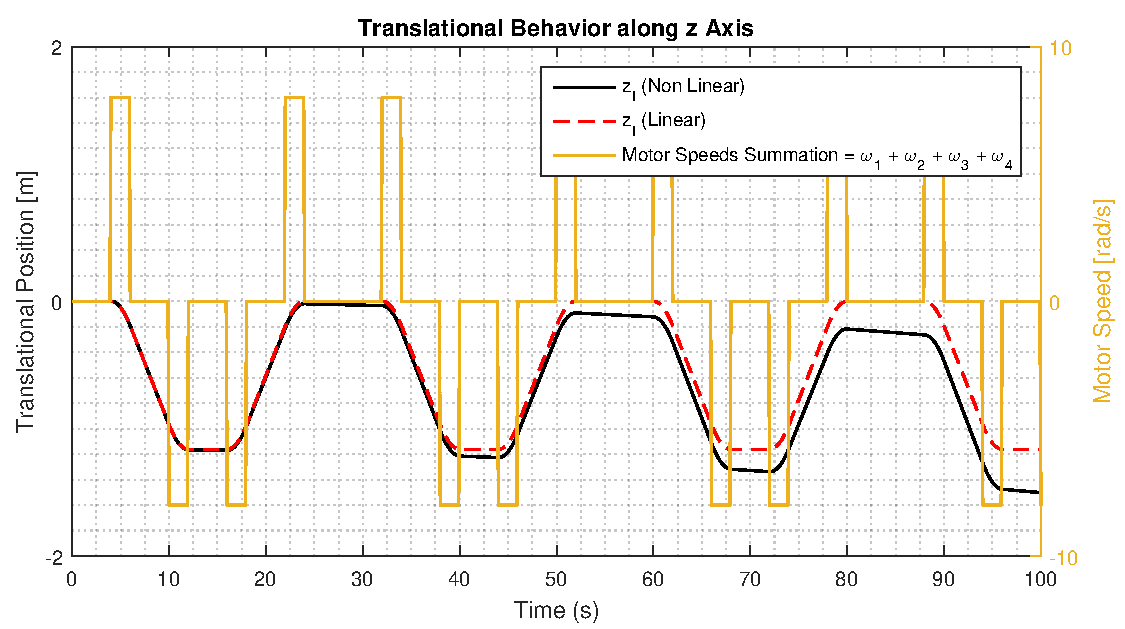
\includegraphics[scale=0.65]{figures/zCompModel}
	\caption{Behavior of the non linear and linear models along the z axis..}
	\label{fig:zCompModel}
\end{figure}

In this chapter, the attitude and translational models of the system have been derived. A linear approximation of the obtained equations will be used in the next chapter to design the necessary controllers to achieve the desired flight behavior for the quadcopter.




